
%%%%%%%%%%%%%%%%%%%%%%%%%%%%%%%%%%%%%%%%%%%%%
%%%%%%%%%%%%%%%STICHPROBE%%%%%%%%%%%%%%%%%%%
%%%%%%%%%%%%%%%%%%%%%%%%%%%%%%%%%%%%%%%%%%%%%

	\section{Stichprobe}\label{stichprobe}
			Die Stichprobe bildet sich aus 40 gesunden Personen zwischen $18$ und $30$ Jahren ($32$ weiblich, $7$ männlich, $1$ divers, $M_{\textrm{Alter}}=24.1$ mit $SD_{\textrm{Alter}}=3.3$).
			Ausschlusskriterien im Zuge der Rekrutierung sind zum einen ein BMI, der kleiner als \SI[per-mode=symbol]{18.5}{\kilogram\per\square\meter} oder größer als \SI[per-mode=symbol]{30}{\kilogram\per\square\meter} ist. Zum Anderen führt das Vorliegen von kardiovaskulären, neurologischen und Atemwegserkrankungen, eingeschränktes Hör- oder Farbsehvermögen, Klaustrophobie, Schwangerschaft oder die Einnahme von bestimmten Medikamenten (kardioaktiv, antidepressiv, antipsychotisch, antihypertensiv oder anticholinerg) zum Ausschluss. Des Weiteren müssen Teilnehmer*innen ein deutsches Sprachverständnis auf mindestens C1-Niveau nachweisen, um an der Studie teilnehmen zu können. 
			Die $n=40$ Versuchspersonen haben zum Zeitpunkt der Datenauswertung mindestens die Akquisitionsphase vollständig durchlaufen. Nicht enthalten in dieser Stichprobe sind Personen, die rekrutiert worden sind, aber noch vor ($n=8$) oder während ($n=1$) %n hier ok?
			des Akquisitionstermins die Teilnahme beendeten. Ein Abbruch nach dem vollständigen Abschluss der Akquisitionsphase ist für diese Arbeit irrelevant und es wurden keine Versuchspersonen aufgrund dessen exkludiert.
			Auf Basis der Datenaufbereitung der Hautleitwert- und Schreckreaktionen (Abschnitt \ref{dataprocessing}) wurden zwei der $40$ Versuchspersonen ausgeschlossen, sodass die finale Analyse mit $n=38$ durchgeführt wurde.
			
			Für den Abschluss der insgesamt vierwöchigen Untersuchung erhalten Teilnehmer*innen eine Aufwandsentschädigung in Form von pauschal $50$ Euro oder $6.5$ bzw. $10.5$ Versuchspersonenstunden bei Zuordnung zur Kontrollgruppe respektive zur Interventionsgruppe (für einen Abbruch nach der Akquisitionsphase wird eine anteilige Entschädigung vergeben).
			Die Rekrutierung der teilnehmenden Personen erfolgt über Aushänge an der Universität, Online-Plattformen und über Beiträge in Sozialen Netzwerken. Jede potentiell geeignete Person durchläuft zu Beginn ein Telefoninterview zur Feststellung der Eignung und wird dabei über den Ablauf der Untersuchung aufgeklärt. Zum ersten Labortermin geben alle Versuchspersonen ihr schriftliches Einverständnis für die Datenverarbeitung und Durchführung der Studie.
			Genehmigt wurde das Projekt durch die Ethikkommission der Universitätsmedizin Greifswald.
			Aufgrund der Ausschlusskriterien und der Einordnung in ein Großprojekt (Abschnitt \ref{hrvbfb}), welches den zeitlichen Rahmen dieser Arbeit weit überschreitet, ist die Stichprobe als eine Gelegenheitsstichprobe zu verstehen.
			

%%%%%%%%%%%%%%%%%%%%%%%%%%%%%%%%%%%%%%%%%%%%%
%%%%%%%%%%%%%%%APPARATUR%%%%%%%%%%%%%%%%%%%%%%%
%%%%%%%%%%%%%%%%%%%%%%%%%%%%%%%%%%%%%%%%%%%%%

	\section{Apparatur}\label{apparatur}
		\subsection{Stimuli}\label{stimuli}
			Die konditionierten Stimuli bilden mit einem blauen Quadrat (Hexadezimalcode: \#00AFF4) und einem orangenen Kreis (\#E46B0C) zwei visuelle geometrische Reize in gleicher Helligkeit. Präsentiert werden diese auf einem schwarzen Hintergrund in der Mitte des Computerbildschirms, jeweils mit einer Dauer von \SI{6}{\second} (für eine Darstellung der Trials siehe Abbildung \ref{fig:ablauf}). Die Intertrial-Intervalle zwischen den Stimuli zeigen ein weißes Fixationskreuz mittig des Bildschirms und variieren in ihrer Länge gleichmäßig zwischen $14$, $15$ und \SI{16}{\second}. Die Reizpräsentation wird über die Software Presentation (Version 20.3, Fa. Neurobehavioral Systems, Inc.) realisiert.
			Welcher der beiden Stimuli den CS+ und welcher den CS-- darstellte, wird über Teilnehmer*innen hinweg ausbalanciert (blaues Quadrat als CS+ $n=21$).
		
			Der CS+ wird partiell durch einen elektrotaktilen Reiz (US) verstärkt, dessen Intensität vor dem Training individuell mit der Versuchsperson eingestellt wird, bis der Reiz als \textit{unangenehm, aber nicht schmerzhaft} bewertet wird ($M=$ \SI{6}{\milli\ampere}, $SD=3.7$, Range $\left[ 1.3;21.0\right]$).
			Die Stimuluselektrode (Stabelektrode, Fa. Technomed GmbH) wird auf der Innenseite des rechten Beins posterior circa \SI{3}{\centi\meter} über dem Knöchel platziert. Kontrolliert wird die elektrische Stimulation über einen DS7A Constant Current Stimulator (Fa. Digitimer, Hertfordshire, UK). Der Ausgangsstrom liegt zwischen $1$ und \SI{100}{\milli\ampere} bei einer Stimulationsdauer von \SI{1}{\milli\second}. Um Habituationsprozesse zu vermeiden, wird die Anzahl der präsentierten US so gering wie möglich gehalten ($M=7.1$ Durchgänge, $SD=4.2$).
	
			Als akustischer Schreckreiz dient ein \SI{50}{\milli\second} langes, \SI{95}{\decibel} weißes Rauschen, welches binaural über Kopfhörer (Modell ATH-PRO700MK2, Fa. Audio-Technica Ltd., Inc.) präsentiert wird. Die Schreckreize werden $4.5$ oder \SI{5.5}{\second} nach jedem CS-Onset und in der Hälfte aller ITI (d.h. $16$ mal) \SI{7.5}{\second} nach CS-Offset verabreicht.
				
		\subsection{EDA- und EMG-Ableitungen}\label{physio}
			Alle physiologischen Ableitungen werden über ein BIOPAC MP160 Verstärker-System und die AcqKnowledge 5.0.2
			Software realisiert (Fa. BIOPAC Systems, Inc., Goleta, CA, USA). %USA? oder deutscher vertrieb? %A/D-Converter: 16 bit
			Eine Erdungselektrode aus Silicon (Fa. TerniMed) wird am linken Oberarm der Versuchsperson befestigt. Alle Elektroden sind wiederverwendbar und werden nach jeder Messung gesäubert und hängend bei Raumtemperatur gelagert. 
			
			Für die EDA-Ableitung wird die nichtdominante Hand der Versuchspersonen zunächst mit Wasser gereinigt. Es werden zwei Ag/AgCl gesinterte Biopotentialelektroden (\SI{8}{\milli\meter} Kontaktflächendurchmesser; Fa. Easycap GmbH) mit isotonischem Elektrodenkontaktgel (\SI{0.5}{\percent} NaCl, GEL101, Fa. BIOPAC Systems, Inc.) gefüllt und anschließend mit doppelseitigen Kleberingen palmarseitig über der Hypothenarmuskulatur angebracht.
			Die Ableitung der EDA erfolgt mit einer EDA100C Komponente (Fa. BIOPAC Systems, Inc.) exosomatisch über ein Konstant-Spannungsverfahren (\SI{0.5}{\volt}). Die EDA-Daten werden kontinuierlich mit einer Abtastrate von \SI[group-minimum-digits = 4]{2000}{\hertz} und einem Verstärkungsfaktor von \SI[per-mode=symbol]{5}{\micro\siemens\per\volt} abgeleitet % Biopac Gain: 5µS/V
			und durchlaufen einen \SI{10}{\hertz} Tiefpassfilter. %Biopac Lowpassfilter: 10hz, HighPass (HP): DC, DC
			%Die Leitfähigkeit wird in Siemens (1 S = 1/Ω) gemessen. Da die Leitfähigkeit der Haut sehr gering ist wird aber meistens μS benutzt (typisch: 2 – 20μS, phasische Veränderung nur 0.02-1μS)
			
			Die Schreckreaktion wird über ein EMG des Orbicularis Oculi Muskels gemessen. Dafür wird die Haut unter dem linken Auge der Versuchsperson mit einem wasserfeuchten Tuch gereinigt. Anschließend werden zwei Ag/AgCl Elektroden (\SI{5}{\milli\meter} Kontaktflächendurchmesser; Fa. Schuler Medizintechnik GmbH) mit Elektrodenkontaktcreme (Electrode Cream, Fa. CareFusion) gefüllt. Diese werden mit doppelseitigen, zugeschnittenen Kleberingen, um sie möglichst nah aneinander zu positionieren, unter dem linken Auge angebracht. Die erste Elektrode liegt dabei circa $0.5$ bis \SI{1}{\centi\meter} unterhalb des Auges lotrecht zur Pupille, die zweite in laterale Richtung daneben (parallel zum Lidverlauf), circa \SI{1}{\centi\meter} vom äußeren Lidwinkel entfernt. 
			Das EMG-Signal wird mit der EMG100C Komponente (Fa. BIOPAC Systems, Inc.) bei einer Abtastrate von \SI[group-minimum-digits = 4]{2000}{\hertz} erhoben. Die Rohdaten des EMG durchlaufen den verstärker-eigenen Bandpassfilter, der Frequenzen zwischen $10$ und \SI{500}{\hertz} passieren lässt, %Der Frequenzbereich des EMG-Verstärkers von Biopac: LP: 500Hz, HP: 10Hz
			und werden um den Faktor $5\,000$ verstärkt. %Gain: 5000
	
			
		\subsection{Zusätzliche Erhebungen}\label{ableitungen}
			Aufgrund des Großprojekts, in dessen Rahmen diese Erhebung läuft, werden zusätzlich zu den obig beschriebenen Ableitungen auch andere abhängige Variablen erhoben, die in dieser Arbeit nicht weiter betrachtet werden. Vor dem Akquisitionstermin füllen die Versuchspersonen einen Fragebogen aus, der verschiedene Elemente u.\,a. aus dem State-Trait-Angstinventar \parencite{STAI} oder dem Brief Symptom Inventory \parencite{BSI} enthält.
			Während der Akquisitionsphase wird außerdem ein Elektrokardiogramm (EKG) aufgezeichnet. Hierfür werden zwei mit Elektrodenkontaktcreme (Electrode Cream, Fa. CareFusion) gefüllte Ag/AgCl-Elektroden (\SI{10}{\milli\meter} Kontaktflächendurchmesser; Fa. Schuler Medizintechnik GmbH) mit doppelseitigen Kleberingen am rechten Unterarm (ca. \SI{2}{\centi\meter} unterhalb der Armbeuge) und am linken Bein (ca. \SI{2}{\centi\meter} proximal des Knöchels) angebracht. Die Ableitung erfolgt endosomatisch ebenfalls über das BIOPAC-System (Fa. BIOPAC Systems, Inc.). 
			Zusätzlich bewerten die Proband*innen vor und nach dem Akquisitionstraining die Valenz und Erregung der präsentierten Stimuli und beantworten nach der Messung kurze Fragen zu ihrem Kontingenzbewusstsein und ihrer Lebensführung. 


%%%%%%%%%%%%%%%%%%%%%%%%%%%%%%%%%%%%%%%%%%%%%
%%%%%%%%%%%%%%%DURCHFÜRHUNG%%%%%%%%%%%%%%%%%%%
%%%%%%%%%%%%%%%%%%%%%%%%%%%%%%%%%%%%%%%%%%%%%

	\section{Durchführung}\label{durchführung}
			\subsection{Einordnung in das Forschungsprojekt}\label{hrvbfb}
						Die Daten werden im Rahmen eines größeren Forschungsprojekts, finanziert von der Deutschen Forschungsgesellschaft, erhoben. Dieses untersucht die Auswirkungen einer Intervention zum Herzratenvariabilität-Biofeedback auf das Extinktionslernen bei gesunden Menschen und bei Personen mit diagnostizierter Panikstörung, Agoraphobie oder beidem. % nach \citetitle{DSM5} (\citefield{DSM5}{edition}; \citefield{DSM5}{shorthand}; \citeauthor{DSM5}, \citeyear{DSM5}). 
						Die Erhebungen laufen an der Universität Potsdam und an der Universität Greifswald unter der Projektleitung von Dr.~Wendt und Dipl.-Psych.  Hufenbach. 
						Im Rahmen der Studie werden die Versuchspersonen über einen Zeitraum von vier Wochen begleitet. Nach einem Labortermin zur Furchtakquisition werden Herzratenparameter der Teilnehmer*innen einmal pro Woche für vier Wochen erfasst. Die gesunden Versuchspersonen der Interventionsgruppe führen während dieser Zeit täglich Übungen zum Stressmanagement mit dem mobilen HRV-Biofeedbackgerät Qiu (Fa. BioSign GmbH) durch. Am Ende der vier Wochen erfolgt ein Labortermin zur Furchtextinktion. 
						Für diese Arbeit werden lediglich die Daten der Akquisitionsphase (am ersten Labortermin) betrachtet und ausschließlich die in Potsdam erhobene Stichprobe der gesunden Versuchspersonen. Weder die Versuchsperson noch die Versuchsleitung weiß zum Zeitpunkt der Akquisitionsphase, welcher der beiden Experimentalgruppen die Person zugeordnet wird. Diese Zuordnung erfolgt erst nach abgeschlossenem Akquisitionstraining und ist somit irrelevant für den Inhalt dieser Arbeit.
						
			\subsection{Anmerkungen zum Erhebungskontext}\label{context}
						Die Datenerhebung begann im Juni 2020 in den peripherphysiologischen Laborräumen der Universität Potsdam und hält zum Zeitpunkt des Verfassens dieser Arbeit noch an. Die Fenster des Experimentalraums sind für den Zeitraum der Erhebung vollständig abgedunkelt, der Raum ist geräuscharm. Die Beleuchtung wird während der Experimentalabschnitte gedimmt, wobei aufgrund technischer Schwierigkeiten die Lichtintensität über die Untersuchungsmonate hinweg geringen Schwankungen unterliegt. Um mögliche Interferenzen durch laute Geräusche zu unterbinden, wird die Klimaanlage während der Messung ausgeschaltet. Die Raumtemperatur beträgt im Mittel \SI{22}{\degreeCelsius} ($SD=1$) bei einer mittleren Luftfeuchtigkeit von $43.2$\si{\percent} ($SD=10$) .
						
						Vor dem Labortermin erhalten alle Versuchspersonen eine E-Mail mit Instruktionen, die vor der Messung einzuhalten sind. Die Proband*innen werden instruiert, am Tag vor dem Termin der Furchtakquisition ihre gewöhnliche Schlafroutine zu verfolgen, auf intensives körperliches Training und Alkohol mindestens \SI{24}{\hour} vor der Messung zu verzichten und im Zeitraum von zwei Stunden vor der Messung keine Mahlzeiten, Koffein oder Nikotin zu sich zu nehmen. Außerdem werden sie gebeten, auf Make-Up im Augenbereich und Strumpfhosen im Sinne der Elektrodenanbringung zu verzichten. 
						
						Die Datenerhebung findet während der globalen Covid-19 Pandemie statt und unterliegt somit verschärften Hygienebestimmungen, die im Hygienekonzept des Bereichs Emotions- und Biopsychologie der Universität Potsdam vom 09.05.2020 festgehalten wurden.
						Die Versuchspersonen und die Versuchsleitung sind verpflichtet, sich vor Beginn der Messung intensiv die Hände zu waschen. Bis auf das Anbringen und Abnehmen der Elektroden wird ein Mindestabstand von \SI{1.5}{\meter} zur Versuchsperson eingehalten. Die Versuchsleiter*innen tragen während des kompletten Erhebungszeitraums einen Mund-Nasen-Schutz sowie zusätzlich ein Gesichtsvisier, wenn der Mindestabstand unterschritten wird. Die Versuchspersonen selbst tragen zu Beginn und zum Ende der Termine ebenfalls einen Mund-Nasen-Schutz, während der Messungen wird aufgrund der EMG-Ableitung am Auge darauf verzichtet. Die maximale Anzahl an Personen in einem Raum wird auf zwei beschränkt, parallele Messungen im angrenzenden EEG-Labor finden nur zu seltenen Ausnahmen statt. Zudem wird eine ausreichende Desinfektion und Reinigung aller mehrfach verwendeten Materialien sowie ausgiebiges Lüften zwischen den Messungen akribisch eingehalten. 
		
						
			\subsection{Vor dem Akquisitionstraining}\label{preacq}

						Zu Beginn werden die Versuchspersonen in den abgedunkelten Laborraum geführt und nehmen auf einem Laborstuhl Platz, dessen Rückenlehne sich in \SI{2}{\meter} %(Potsdam) oder \SI{1.55}{\meter} (Greifswald)
						Entfernung zu einem Computerbildschirm (Modell VG275Q, Fa. ASUSTeK Computer, Inc.) befindet. Die Proband*innen werden über den Ablauf der Untersuchung informiert und geben ihr schriftliches Einverständnis. 	
					%HRV RUHEMESSUNG					
						Nach Anbringen der EKG-Elektroden findet eine sechsminütige Ruhemessung der Herzratenvariabilität statt. Die Versuchspersonen werden verbal instruiert, entspannt und möglichst bewegungsarm mit geschlossenen Augen im Laborstuhl zu sitzen.
						Danach werden die EDA- und EMG-Elektroden (Abschnitt \ref{apparatur}) angebracht. EKG-, EDA- und EMG-Daten werden bis zum Ende des Akquisitionstrainings ununterbrochen aufgezeichnet, was ca. \SI{40}{\minute} entspricht.
					%STARTLE HABITUATION
						Es folgt eine Habituation der Schreckreaktion, bei der die Versuchspersonen ein weißes Fixationskreuz in der Mitte des schwarzen Computerbildschirms fixieren sollen, während ihnen der akustische Schreckreiz vier Mal präsentiert wird. Sie werden instruiert, dabei keine besondere Aufgabe zu haben. %Die Stimuli werden $5$, $16$, $29$ und $44$ Sekunden nach Beginn des Untersuchungsabschnittes ausgelöst und die Reaktionen auf allen drei physiologischen Reaktionsebenen (EKG, EMG, EDA) erfasst. 
												
					%INTENSITÄT US
						Danach erfolgt die individuelle Einstellung des elektrotaktilen Reizes. Zunächst werden die Versuchspersonen über das Vorgehen aufgeklärt, im Anschluss wird die Stimulationselektrode angebracht. 						
						Für den Kalibrierungsprozess erhalten die Versuchspersonen eine Computermaus und eine $5$-stufige Skala in laminierter Form (von \textit{Gar nicht unangenehm} bis \textit{Schmerzhaft}; \nameref{appA}1).
						Auf dem Computerbildschirm erscheint eine Instruktion in Textform mit dem Wortlaut: "`Drücke die linke Maustaste für den Reiz. Dieser folgt dann $3$ Sekunden später"'.
						Die Versuchspersonen lösen den elektrotaktilen Reiz im Einstellungsprozess immer eigenständig aus und schätzen nach jedem Reiz auf der ausgeteilten Skala ein, wie unangenehm er für sie war. Die Tür zum Kontrollraum, in dem die Versuchsleitung die Reizeinstellung verändert und dokumentiert, bleibt dabei offen, sodass eine direkte Kommunikation mit den Versuchspersonen möglich ist. 
						Die Intensität des elektrotaktilen Reizes startet bei \SI{1}{\milli\ampere} und wird sequentiell in Abhängigkeit des Ratings erhöht oder verringert, bis die Personen den Reiz als \textit{unangenehm, aber nicht schmerzhaft} einschätzen, was auf der Skala dem Rating $4$ entspricht (\nameref{appA}2 enthält die Tabelle zur Kalibrierung). Diese Intensität wird als final eingestellt und dokumentiert.
									
					%PRE- FURCHTAKQUISITIONSTRAINING
						Anschließend werden den Versuchspersonen auf dem Computerbildschirm die beiden visuellen Stimuli (Abschnitt \ref{stimuli}) nebeneinander präsentiert. Die Proband*innen werden aufgefordert, die Stimuli verbal hinsichtlich ihrer Valenz und Erregung einzuschätzen. Dazu dienen Self-Assessment-Manikin Skalen für Valenz und Erregung \parencite[SAM;][]{BRADLEY1994}, denen aufsteigend absolute Zahlen von $1$ bis $9$ zugeordnet werden (\nameref{appB}).
	
			
			\subsection{Akquisitionstraining}\label{acq}		
			
					 	Für das Akquisitionstraining erhalten die Versuchspersonen verbal die Instruktion, ruhig mit offenen Augen sitzen zu bleiben und den Computerbildschirm aufmerksam zu beobachten. Sie werden darauf hingewiesen, dass ihnen neben den visuellen Reizen auch akustische Stimuli und elektrotaktile Reize dargeboten werden können. Außerdem wird ihnen mitgeteilt, dass der nächste Abschnitt mit akustischen Reizen beginne, auf die sie nicht zu achten brauchten und dass sie keine besondere Aufgabe hätten.
					 	Das Furchtakquisitionstraining beginnt mit vier Schreckreizen und besteht danach aus insgesamt $32$ Trials. Beide CS werden jeweils $16$ Mal in ausbalancierter Reihenfolge in Viererblöcken präsentiert, sodass nicht mehr als zwei gleiche Reize direkt aufeinander folgen. Das Verhältnis der Stimuli innerhalb der Blöcke bleibt dabei gleich. Auf den CS+ folgt in \SI{50}{\percent} aller Fälle ein US (d.h. acht verstärkte Trials), während der CS-- niemals verstärkt wird. Das Design entspricht einer Verzögerungskonditionierung mit einem Interstimulus-Intervall von \SI{5.95}{\second}, sodass der US kurz vor dem CS-Offset verabreicht wird. 
					 		\begin{figure}[h]
					 			\begin{center}
					 			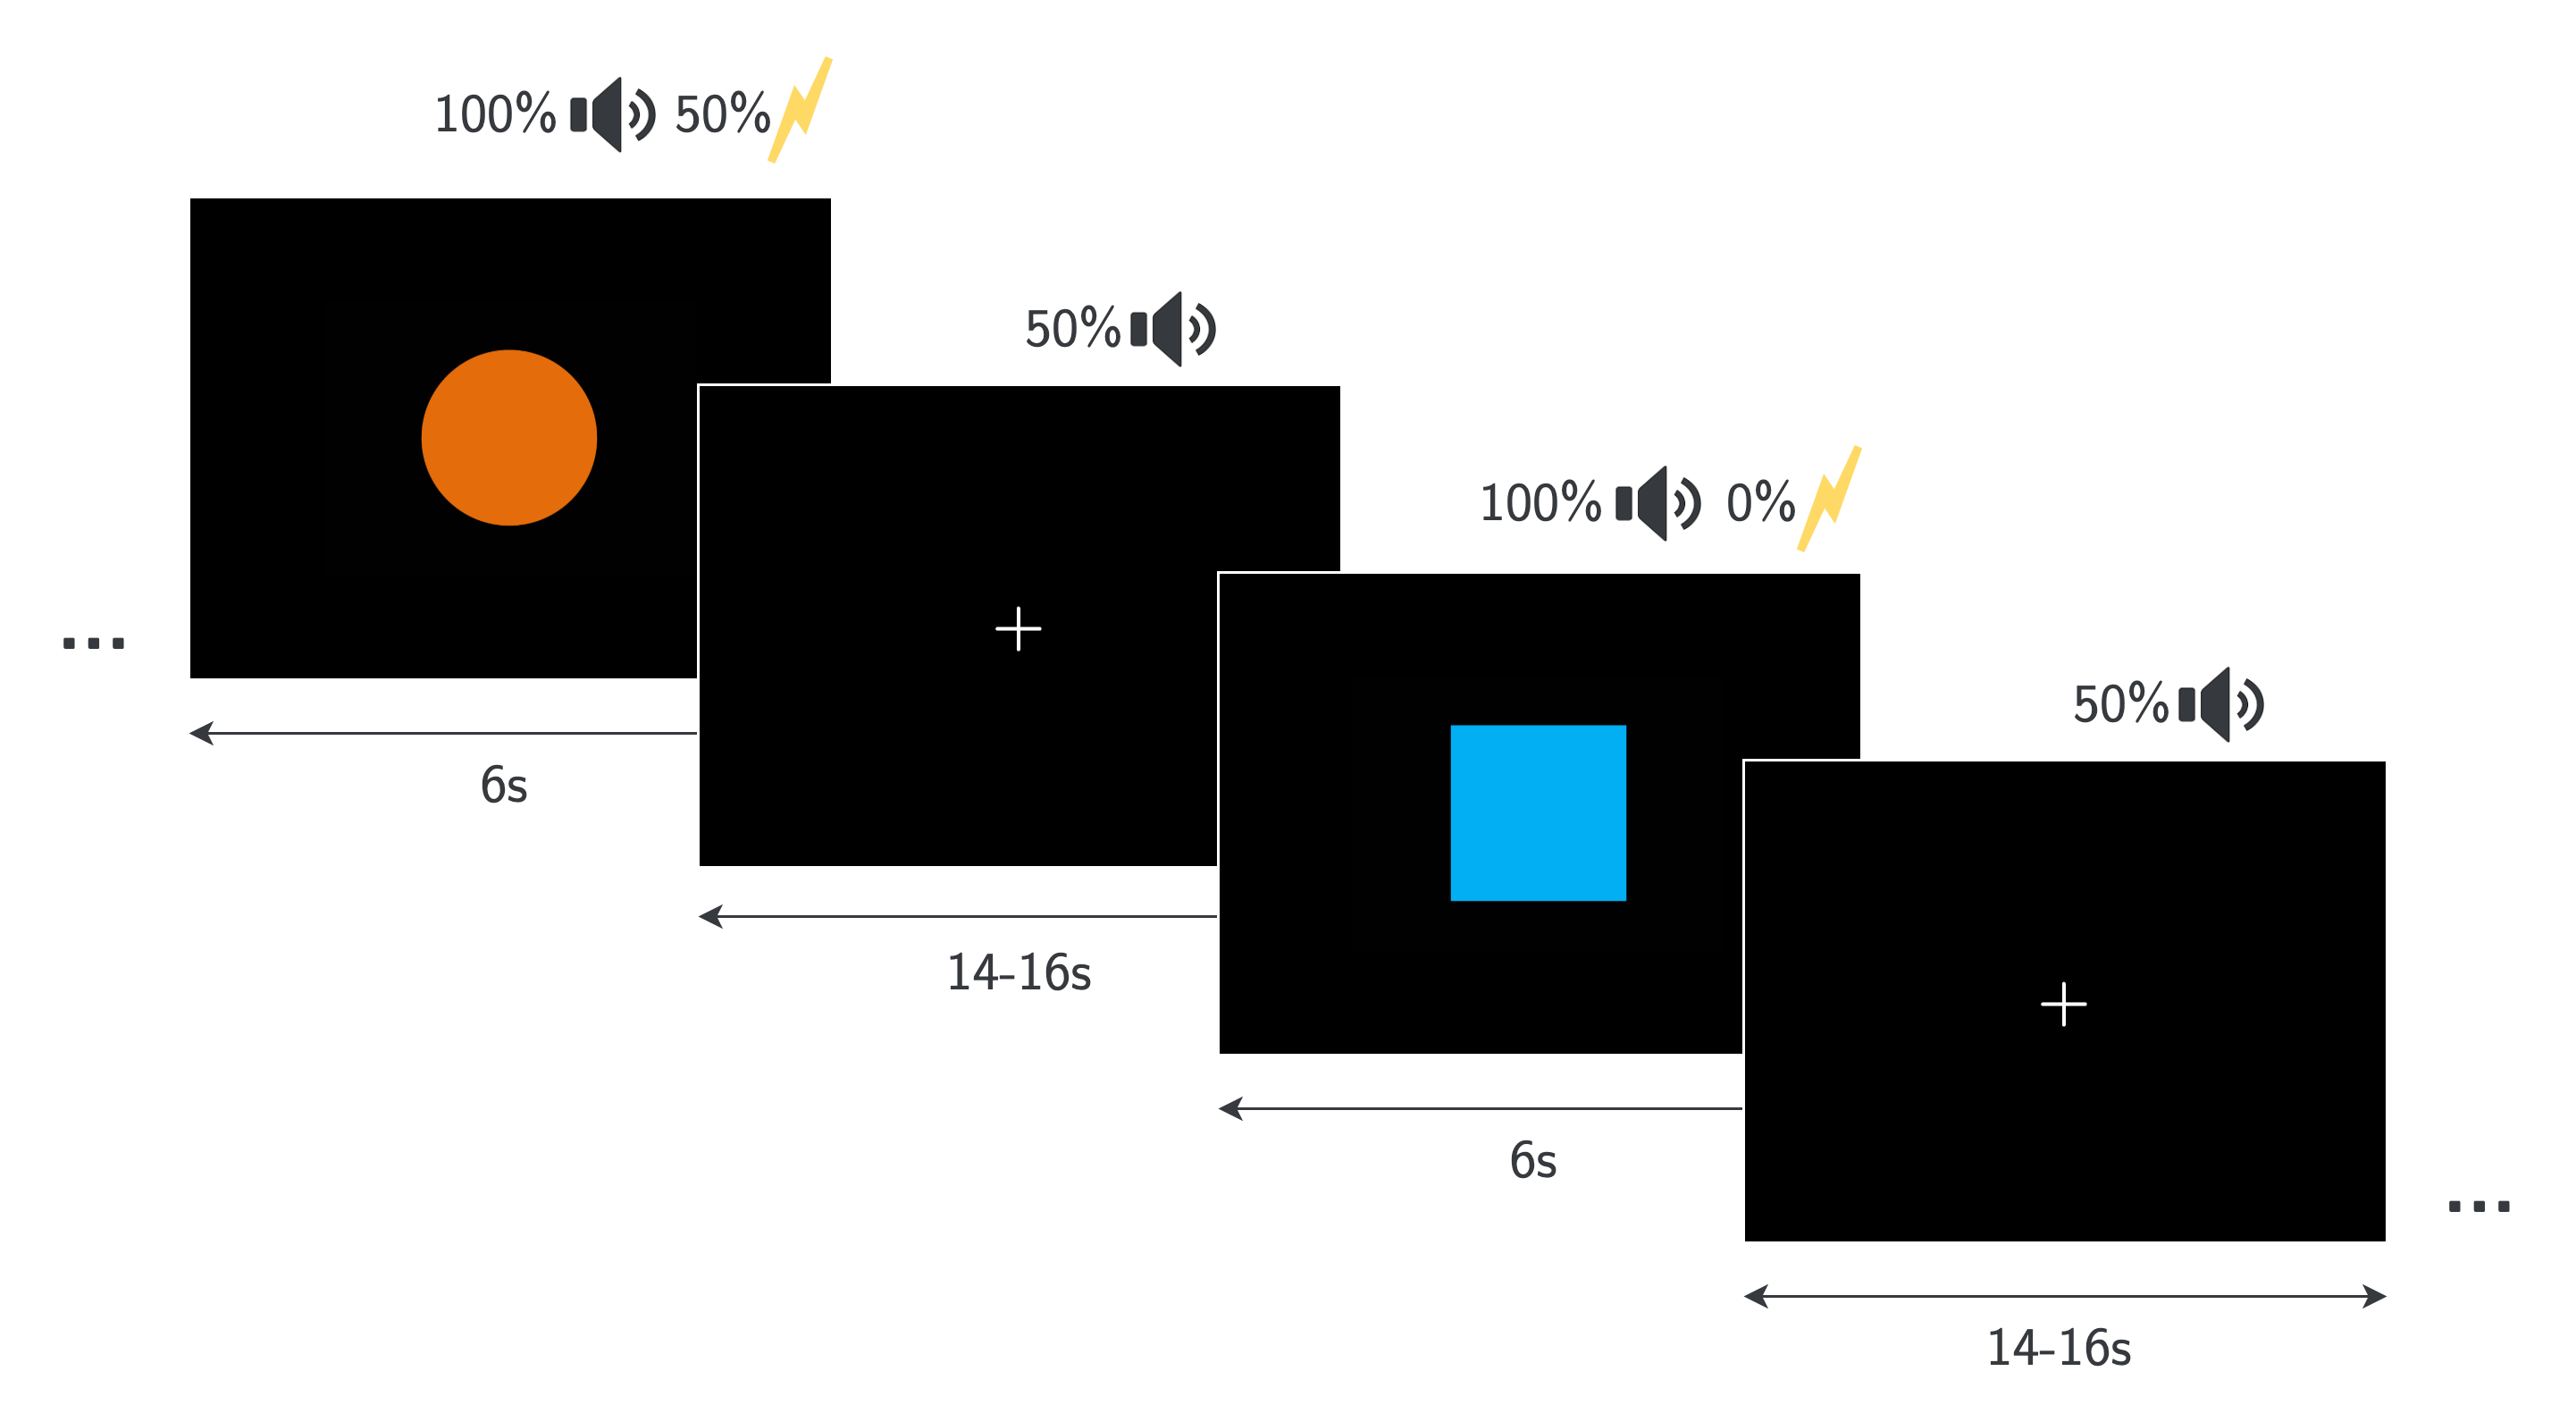
\includegraphics[width=0.9\textwidth]{ablauf.png}
					 			\caption[Schematischer Ablauf der Trials]{Schematischer Ablauf der Trials (exemplarisch: orangener Kreis als CS+). Die Prozente entsprechen den Wahrscheinlichkeiten für die Vergabe von Schreckreizen und elektrotaktilen Reizen in den jeweiligen Trials.}
					 			\label{fig:ablauf}
					 	\end{center}\end{figure}
				 	
						Die Versuchspersonen werden auf jeweils einer von vier verschiedenen Trialreihenfolgen getestet, deren wesentliche Unterschiede darin liegen, mit welchen Stimuli das Akquisitionstraining beginnt (CS+ oder CS--) und ob der erste präsentierte CS+ verstärkt wird oder nicht. Die Reihenfolgen werden über Versuchspersonen hinweg ausbalanciert. 
						In der Hälfte des Trainings nach dem $16.$ Trial wird eine vollständige Instruktion auf dem Bildschirm präsentiert. Mit dem Wortlaut "`Wenn ein unangenehmer Reiz am Bein erfolgt, dann immer nur bei diesem Symbol:"' und einer Abbildung des CS+ werden die Versuchspersonen über die CS-US-Kontingenz aufgeklärt.
						Grund für die Darbietung der Instruktion ist einerseits die Fokussierung des Großprojekts auf den Extinktionstermin, für den eine gelernte CS-US-Kontingenz unabdingbar ist, und andererseits die anteilige Messung der Patient*innen-Stichprobe.
						
					%POST- FURCHTAKQUISITIONSTRAINING
						Das Akquisitionstraining insgesamt dauert ca. \SI{12}{\minute}. Im Anschluss werden die Proband*innen erneut um eine Einschätzung aller präsentierten Reize (CS+, CS--, Auslösereiz, US) auf den SAM-Skalen (\nameref{appB}) gebeten. Es folgt ein kurzes Bewusstseins-Interview, bei dem erfasst wird, ob die Versuchspersonen eine Regel in Bezug auf die CS-US-Kontingenz verbalisieren können. An dieser Stelle wird von der Versuchsleitung sichergestellt, dass die Kontingenz spätestens nach Abschluss des Trainings bekannt ist. Dieses halb-standardisierte Interview soll eine erfolgreiche Furchtakquisition bei allen Versuchspersonen gewährleisten, um den für das Großprojekt relevanten Extinktionstermin durchführen zu können. 
						Nach einigen kurzen Fragen zu Mahlzeiten, Koffein- und Alkoholkonsum vor der Messung werden die Versuchspersonen an die Interventionsleitung übergeben. Dort werden sie über ihre Zugehörigkeit zu Kontroll- bzw. Interventionsgruppe aufgeklärt und im Zuge des Großprojekts weiter begleitet.
					 

%%%%%%%%%%%%%%%%%%%%%%%%%%%%%%%%%%%%%%%%%%%%%%%%
%%%%%%%%%%%%%%%PREPROCESSING%%%%%%%%%%%%%%%%%%%%
%%%%%%%%%%%%%%%%%%%%%%%%%%%%%%%%%%%%%%%%%%%%%%%%

	\section{Datenverarbeitung und Reaktionsdefinition}\label{dataprocessing}

		\subsection{Hautleitwertreaktion}\label{edascore}
			
			Die Vorverarbeitung sowohl der EDA- als auch der EMG-Daten erfolgt in \citeauthor{MATLAB} (Version R2020b, MathWorks, Inc., Natick, USA).	
			Die EDA-Daten werden offline auf \SI{100}{\hertz} heruntergetaktet. Die Vorverarbeitung und Kennwertbestimmung der Daten erfolgt mit der Ledalab Software V3.4.9 \parencite{BENEDEK2010} nach veröffentlichten Richtlinien \parencite{BOUCSEIN2012}. Dabei wird automatisch im Zeitfenster von $0.9$ bis \SI{5}{\second} nach CS-Onset eine klassische Tiefpunkt-bis-Hochpunkt Differenz gebildet, wobei eine Mindestamplitude von \SI{0.001}{\micro\siemens} als Wertungskriterium dient. Die Hautleitwertreaktion entspricht damit der jeweiligen Amplitudenhöhe in~\si{\micro\siemens}. Dadurch, dass der Schreckreiz frühestens \SI{4.5}{\second} nach CS-Onset präsentiert wird und eine SCR auf diesen erst eine Sekunde ihren  Onset hätte, interferiert die Vergabe des Schreckreizes nicht mit der Erfassung der SCR in diesem Zeitfenster.
			Nach der Verarbeitung in Ledalab werden die Gesamtreaktionen der einzelnen Versuchspersonen manuell inspiziert. In $n=2$ Fällen sind keine SCR-Reaktionen im Akquisitionstraining erfasst worden, vermutlich aufgrund des Ablösens der Elektroden während der Messung. Diese beiden Versuchspersonen werden aus allen Folgeanalysen ausgeschlossen.
			Nullreaktionen werden vergeben, wenn die Amplitude der SCR das Mindestkriterium nicht erfüllt. Die übrigen $38$ Datensätze enthalten \SI{18}{\percent} ($223$ von $1\,216$) Nullreaktionen. Fehlende Reaktionen gibt es aufgrund der automatischen Auswertung nicht.
			Auf Basis der Empfehlung eines durchgeführten Box-Cox-Tests für die SCR-Daten wird eine log-Transformation dieser Daten vorgenommen \parencite{BOX1964}.
			%Ledalab Optimizer Nr. 4 (Number of different sets of initial values) einbringen?
			%19.03. finale Analyse: Downsample Faktor 20, Time-Window 0.9-5, Kriterium: 0.001µS, 
		
		\subsection{Schreckreaktion}\label{emgscore}
				
			Die EMG-Daten werden offline in \citeauthor{MATLAB} durch einen Hochpassfilter mit \SI{60}{\hertz} und einen Tiefpassfilter mit \SI{400}{\hertz} geschickt (Butterworth Filter zweiten Grades, \nptextcite{BLUMENTHAL2005}) %60Hz Hochpassfilter, 400Hz Tiefpassfilter --> %alternativ: Breitbandfilter mit Grenzen 60 und 400?
			und durchlaufen zusätzlich einen Kerbfilter bei \SI{50}{\hertz}, um Interferenzen durch Netzbrummen zu reduzieren. % 50Hz Bandstop Filter
			Das Signal wird gleichgerichtet und mit einem Tiefpassfilter von \SI{15.9}{\hertz} und einer Zeitkonstante von \SI{10}{\milli\second} geglättet. %OrbicularisRect= abs(OrbicularisFilt) und OrbicularisIntegratedDef= filter(tp10ms,OrbicularisRect)
			Die Kennwertbestimmung erfolgt manuell, indem innerhalb von $20$ bis \SI{120}{\milli\second} nach dem Schreckreiz der Fußpunkt der Reaktion und innerhalb von \SI{150}{\milli\second} das lokale Maximum als Spitze festgelegt werden \parencite{BLUMENTHAL2005}. Die Schreckreaktion ergibt sich aus der Differenz (d.\,h. der Amplitudenhöhe) in~\si{\micro\volt}.
			Trials, die eine exzessive Grundlinienaktivität oder ein zufälliges Blinzeln kurz vor oder zu Beginn des interessierenden Zeitfensters zeigen, werden als \textit{fehlend}  definiert. Von allen Trials sind $13$ (\SI{1.1}{\percent}) fehlend (wobei keine Versuchsperson mehr als zwei fehlende Werte aufweist). 
			Für Trials, in denen eine Reaktion nicht distinkt erkennbar ist bzw. vollständig ausbleibt, wird eine Nullreaktion vergeben. Die Anzahl der Nullreaktionen beläuft sich auf $19$ (\SI{1.6}{\percent}), wobei anzumerken ist, dass kein Kriterium für eine Mindestreaktionshöhe einer vorhandenen Reaktion angelegt wird.
			%Der Mittelwert und die Standardabweichung der Schreckreaktionen innerhalb der Versuchspersonen wurden berechnet und die Schreckreaktionen anhand dieser Werte z-standardisiert. 
	
	
%%%%%%%%%%%%%%%%%%%%%%%%%%%%%%%%%%%%%%%%%%%%%%%%%%%
%%%%%%%%%%%%%%%STATISTISCHE ANALYSE%%%%%%%%%%%%%%%%
%%%%%%%%%%%%%%%%%%%%%%%%%%%%%%%%%%%%%%%%%%%%%%%%%%%
\section{Statistische Analyse}\label{statistik}
	
	\subsection{Multivariates Wachstumsmodell mit Mehrebenenstruktur}
		Der statistische Vergleich findet durch ein multivariates Wachstumsmodell (engl.: Growth Curve Analysis) im Rahmen eines Mehrebenenmodells statt. 
		Mehrebenenmodelle (MEM) haben sich in den letzten Jahren psychophysiologischer Forschung zunehmend durchgesetzt, da sie für messwiederholte Daten als flexibler und präziser gelten. Als Erweiterung der regulären Regression können mit ihnen Daten analysiert werden, denen eine Mehrebenenstruktur zugrunde liegt (man spricht häufig von einer Hierarchie oder Verschachtelung der Daten).
		Im Fall dieser Arbeit besteht die Mehrebenenstruktur darin, dass für jede Versuchsperson eine Vielzahl an Messungen (mehrere Trials) erhoben wird und die einzelnen Beobachtungen einer Person nicht als unabhängig voneinander anzusehen sind.
		 
		Üblicherweise verwendete statistische Verfahren wie die messwiederholte ANOVA oder Regressionen mit Ordinary-Least-Squares Schätzungen (dt.: Methode der kleinsten Quadrate) können für diese Datenstruktur nicht aufkommen und führen zu verfälschten Schätzparametern und Signifikanztests \parencite{NEZLEK2012}. 
		MEM währenddessen erlauben den Regressionsparametern wie dem Intercept (dt.: Achsenabschnitt) und den Slopes (dt.: Steigungen) zwischen den Ebenen zu variieren. Damit schätzen sie Regressionskoeffizienten nicht nur als feste Effekte (engl.: fixed effects), sondern modellieren sie als zufällige Effekte (engl.: random effects). Die festen Effekte sind ähnlich wie in herkömmlichen Regressionsmethoden zu verstehen.
		Mit der zusätzlichen Schätzung der Zufallsfehler dieser festen Koeffizienten ist es den Regressionsparametern der einzelnen Personen im Modell nun aber \textit{erlaubt}, von diesem mittleren Effekt abzuweichen. Die Modellierung als zufällige Effekte repräsentiert die Annahme, dass die geschätzten Regressionsparameter Stichproben aus einer zugrundeliegenden Verteilung von Parametern in der Grundgesamtheit sind.
		Die simultane Schätzung von Zufallsfehlern nicht nur auf Ebene der Reaktion (Ebene 1), sondern auch auf Ebene der einzelnen Versuchsperson (Ebene 2) ist ein wesentlicher Vorteil von MEM. Vor allem in der Psychophysiologie, wo es zwischen verschiedenen Personen zu enormen Schwankungen in Reaktionsmustern kommen kann, zeigen MEM die notwendige Flexibilität, bessere Erklärungen für ihre Datenmuster bereitstellen zu können.
		Zusätzlich bieten MEM den Vorteil, für eine fehlende Äquidistanz von Messzeitpunkten aufzukommen sowie mit fehlenden Datenpunkten umzugehen (ungleich üblicher ANOVA-Methoden) und damit reliablere Schlussfolgerungen zu liefern. 	
		
		Im Kontext von messwiederholten Daten, denen eine zeitliche Struktur zugrunde liegt, erlauben diese Modelle die Schätzung von sogenannten \textit{Wachstumskurven}. Dieser eher breite Term umfasst im MEM-Kontext die Untersuchung von intraindividuellen Veränderungen und den Prädiktoren, die diese beeinflussen können \parencite{CURRAN2010}.
		Eine tiefgehende Erläuterung der Konzepte von Wachstumskurven- und Mehrebenenanalysen geht über den Umfang dieser Arbeit weit hinaus. Eine englischsprachige Einführung in die Thematik geben zum Beispiel \textcite{BAGIELLA2000, NEZLEK2012} und \textcite{PAGEGOULD2016}, als deutschsprachige Einführung eignet sich \textcite{NEZLEK2006}. Für einen tieferen Einblick seien die Bücher von \textcite{GRIMM2017, BICKEL2007} und \textcite{RAUDENBUSH2002} empfohlen. 
		Um einen Vergleich zweier abhängiger Variablen zu implementieren, wird das univariate Wachstumsmodell auf ein multivariates erweitert \parencite[nach dem Vorbild von][]{CURRAN2012, MACCALLUM1997}. 
		Zusätzlich zu der Schätzung von Wachstumsmodellen für jede der beiden abhängigen Variablen erlaubt der multivariate Ansatz die Untersuchung ihrer Kovarianzen. 
		%Hier kann für jeden der Prädiktoren einzeln der Einfluss auf die Anpassungsgüte geschätzt werden und das wiederum separat für jede der abhängigen Variablen.
		Im Folgenden erläutere ich die in dieser Arbeit umgesetzte Modellstruktur sowie das allgemeine Vorgehen, die Annahmen und die Entscheidungskriterien zum Aufstellen und Schätzen des Modells.
		

	\subsection{Modellstruktur \& Variablen}
		
		Die Daten werden als Zwei-Ebenen-Modell analysiert mit der Reaktion auf Ebene 1 und der Versuchsperson auf Ebene 2. Das heißt, dass jede Reaktion der Versuchsperson zugeordnet wird, von der sie stammt. 
		%Für jede dieser Versuchspersonen wird damit ein individuelles Wachstumsmodell geschätzt für jede der abhängigen Variablen separat und zusätzlich der Einfluss des Stimulustyps und seiner Interaktion mit der Zeit untersucht.
		Einen Überblick über die Datenstruktur liefert Abbildung \ref{fig:struktur}.
		
		\begin{figure}[h]
			\begin{center}
				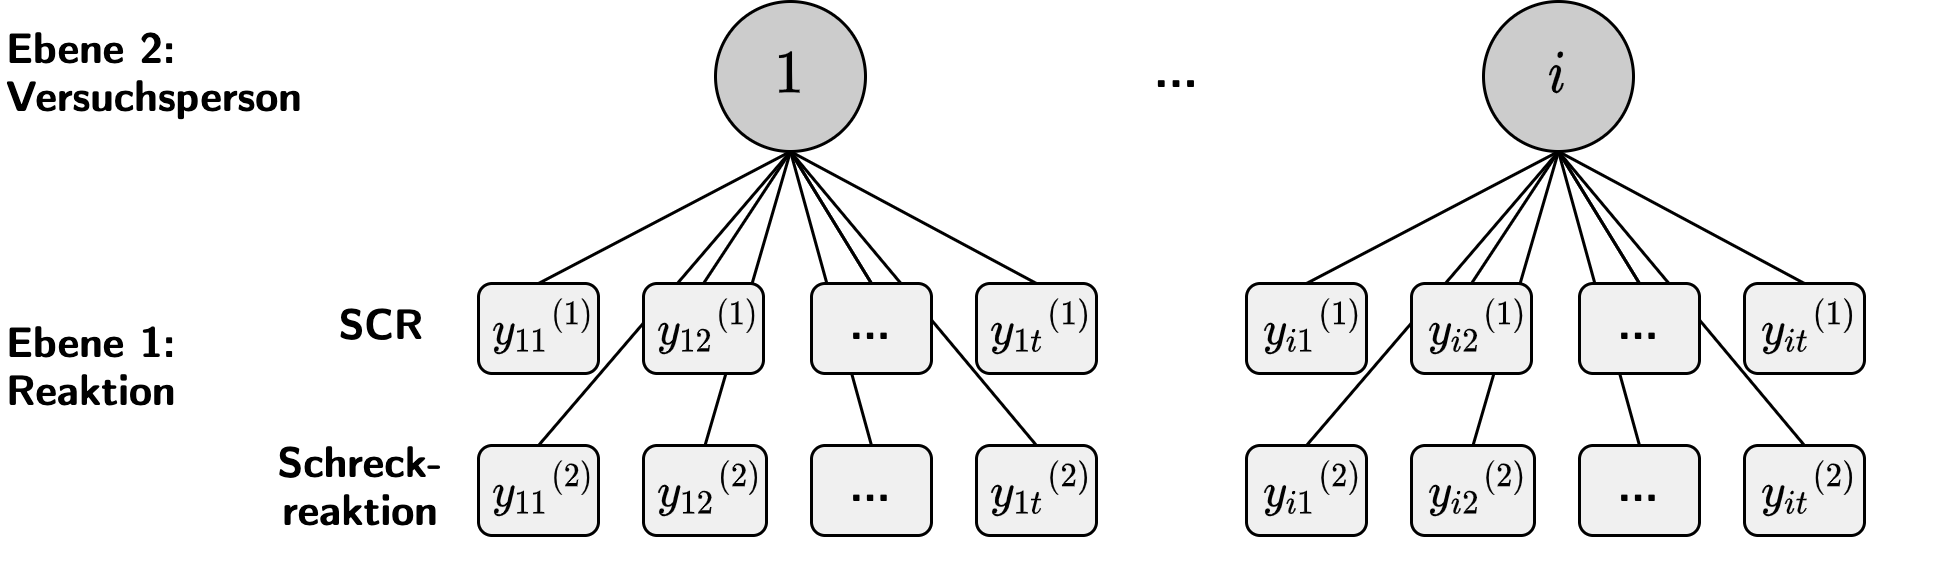
\includegraphics[width=0.8\textwidth]{structure.png}
				\caption[Schematische Datenstruktur im Rahmen des Mehrebenenmodells]
				{Schematische Datenstruktur im Rahmen des Mehrebenenmodells mit zwei Ebenen und zwei abhängigen Variablen ($i$: Versuchsperson, $t$: Trial).}
				\label{fig:struktur}
		\end{center}\end{figure}

		Um ein Wachstumsmodell aufzustellen, benötigt es eine Zeitvariable. In dieser Arbeit wird die Trialnummer als kontinuierlicher Prädiktor herangezogen, um Veränderungen über die Zeit zu erfassen. Bei der Modellbildung wird getestet, ob das Datenmuster der beiden Reaktionsvariablen durch eine lineare oder eine quadratische Zeitvariable besser erklärt werden kann. Dafür wird im Modell ein Polynom-Term zweiten Grades linear-additiv in das Modell inkludiert und sein Effekt auf die Anpassungsgüte überprüft. 
		Um der Multikollinearität der Zeitprädiktoren vorzubeugen, wird die Trialnummer zentriert und anschließend für den quadratischen Modellterm quadriert. Damit liegt der Mittelpunkt der Trialvariable zwischen dem 8. und 9. Trial \parencite[analog zu][]{KRISTJANSSON2007}.
		Der Stimulustyp wird als zweistufiger kategorialer Prädiktor dummykodiert mit dem CS-- als Referenzkategorie. Da jede Versuchsperson sowohl auf den CS+ als auch auf den CS-- in beiden Reaktionsmaßen reagiert, gilt der Stimulustyp als ein sogenannter zeitvarianter Prädiktor, der auf Reaktionsebene des Modells hinzugefügt wird.
		Das multivariate Wachstumsmodell enthält schließlich ebenfalls eine Variable, die kodiert, zu welchem Reaktionsmaß eine Reaktion gehört. Es untersucht den individuellen Verlauf der beiden abhängigen Variablen und kann zusätzlich die Kovariationen zwischen den Koeffizienten dieser beiden Wachstumsmodelle schätzen \parencite{GRIMM2017}. Die Besonderheit ist, dass für jede Person ein eigenes Wachstumsmodell für die Hautleitwert- und die Schreckreaktion geschätzt wird, indem die jeweilige Reaktionsvariable in Abhängigkeit von der Zeit und gegebenenfalls vom Stimulustyp bestimmt wird.
		Die Modellbildung erfolgt mit den unstandardisierten Werten beider Variablen. %xxx ggf: 
		%für den Vergleich der Parameter zwischen den Reaktionsvariablen wird das finale Modell zusätzlich einmal mit standardisierten Werten geschätzt, wobei jeweils der Gesamtmittelwert und die Standardabweichung der Werte genutzt werden.
		Die Tabelle \ref{tab:structure} zeigt exemplarisch die Struktur des Datensatzes in langem Format einschließlich der Kodierung und Zentrierung der Prädiktorvariablen.
		\begin{table}[hbt] \small \setstretch{1.5}
			\begin{threeparttable}
				\caption{Exemplarische Datenstruktur}			%ohne Punkt
				\label{tab:structure}
				\begin{tabularx}{\textwidth}{CCCCCCCC}         \toprule	
					VP  & Reihenfolge & Trial & lin  & quad  & CS & AV  & Reaktion \\\hline
					\rowcolor[HTML]{EFEFEF}
					1   & 3     & 1     & -7.5 & 56.25 & 0        & SCR & 0.0059   \\
					1   & 3     & 1     & -7.5 & 56.25 & 0        & STR & 61.421   \\\rowcolor[HTML]{EFEFEF}
					1   & 3     & 1     & -7.5 & 56.25 & 1        & SCR & 1.5482   \\
					1   & 3     & 1     & -7.5 & 56.25 & 1        & STR & 29.184   \\\rowcolor[HTML]{EFEFEF}
					1   & 3     & 2     & -6.5 & 42.25 & 0        & SCR & 0.0024   \\
					1   & 3     & 2     & -6.5 & 42.25 & 0        & STR & 49.147   \\\rowcolor[HTML]{EFEFEF}
					1   & 3     & 2     & -6.5 & 42.25 & 1        & SCR & 0.2949   \\
					... & ...   & ...   & ...  & ...   & ...      & ... & ... \\[-0.2em]\bottomrule 
				\end{tabularx}
				\begin{tablenotes}[normal, flushleft, para]
					\footnotesize{
						\item \textit{Anmerkungen.} VP: Versuchsperson, Reihenfolge: Zuordnung der Trialreihenfolge, lin: linearer zentrierter Zeitterm, quad: quadrierter zentrierter Zeitterm, CS: Stimulustyp (1: CS+, 0: CS--), AV: abhängige Variable (SCR: Hautleitwertreaktion, STR: Schreckreaktion).}
				\end{tablenotes}
			\end{threeparttable}
		\end{table}
		
		\subsection{Allgemeines Vorgehen bei der Modellbildung}
		
		Der Modellbildungsprozess läuft in mehreren Schritten ab. Nach einer deskriptiven und visuellen Analyse der Reaktionsvariablen wird in Schritt 0 zunächst ein unkonditioniertes Modell aufgestellt, welches keinerlei Prädiktoren enthält. Dieses sogenannte \textit{Nullmodell} dient dazu, die Variabilität zu erfassen, die auf Unterschiede der Versuchspersonen zurückgeführt werden kann. 
			\begin{alignat*}{3}
				\text{Ebene 1} &\qquad\qquad& y_{it}{}^{(k)}&=  	\uppi_{0i}{}^{(k)}+e_{it}{}^{(k)}&\qquad\qquad
			%\tag{2}
			\nr\label{eq:null1}\\
				\qquad\text{Ebene 2} && \uppi_{0i}{}^{(k)}&=  \upbeta_{00}{}^{(k)}+r_{0i}{}^{(k)}&\qquad\qquad \notag
			\end{alignat*}
		In diesem Nullmodell ist $y$ die Reaktion der Versuchsperson $i$ zum Zeitpunkt $t$ auf der Reaktionsvariable $k$. Der Index $k$ beschreibt für $k=1$ die Hautleitwertreaktion und für $k=2$ die Schreckreaktion. Der Modellterm $\uppi_{0i}{}^{(k)}$ ist der individuelle Intercept der Person $i$ auf der Variable $k$.
		Das Residuum $e_{it}{}^{(k)}$ erfasst die Abweichung der Reaktion $y$ vom individuellen Mittelwert, wiederum jeweils für beide $k$. 
		Ebene~2 enthält die Gleichung, mit der der Intercept als zufälliger Effekt modelliert wird. Das Residuum $r_{0i}{}^{(k)}$ gibt an, wie der personenspezifische Intercept vom globalen (festen) Intercept $\upbeta_{00}{}^{(k)}$ abweicht.
		Diese Mehrebenengleichungen lassen sich auch in einem gemischten Format (d.\,h. innerhalb einer Gleichung für beide abhängigen Variablen) kombinieren. Um das zu realisieren, werden zwei zusätzliche Dummyvariablen benötigt – eine für jedes Reaktionsmaß. Diese kodieren, zu welcher abhängigen Variable eine Reaktion zugeordnet werden kann \parencite{MACCALLUM1997}.
		\begin{align*}		
			\updelta_1 = \begin{cases}
				1  & \text{ wenn } k=1 \text{ (Hautleitwertreaktion)}\\
				0  & \text{ wenn } k=2 \end{cases} 
			\qquad \text{und} \qquad \updelta_2 = \begin{cases}
				1  & \text{ wenn } k=2 \text{ (Schreckreaktion)}\\
				0  & \text{ wenn } k=1\end{cases} \nr\label{eq:delta}
		\end{align*}
		Mit der Wichtung über die Dummyvariablen ist es möglich, ein einziges Modell zu schätzen und dabei separate Wachstumsmodelle für die jeweiligen Reaktionsmaße sowie ihre geteilte Varianz zu bestimmen. Dabei kann das Modell trotz einer multivariaten Zwei-Ebenen-Struktur mit derselben Linearkombination geschätzt werden. Für ein gegebenes $y_{it}{}^{(1)}$ zum Beispiel gewährleistet die Variable $\delta$, dass der zweite Summand der Summe aus der Gleichung \eqref{eq:null2} entfällt. In der Summenschreibweise werden damit für  $m=1$ die Regressionsparameter der Hautleitwertreaktion ($k=1$) und für $m=2$ die der Schreckreaktion ($k=2$) geschätzt.
		\begin{equation*}
			y_{it}{}^{(k)}=\sum^2_{m=1} \updelta_m \left( \upbeta_{00}{}^{(m)}+ 		
			r_{0i}{}^{(m)}+e_{it}{}^{(m)}\right)\nr\label{eq:null2}
		\end{equation*}
	
		In Schritt 1 wird die Struktur der zufälligen Effekte bestehend aus zufälligen Intercepts und Slopes für jedes Reaktionsmaß festgelegt. 
		Dafür wird zunächst die maximale Struktur festgestellt (d.h. jeder Regressionskoeffizient wird als zufällig modelliert; \nptextcite{BARR2013}).
		In der maximalen Struktur sind neben zufälligen Intercepts außerdem zufällige Slopes für beide Zeitterme, den Stimulustyp und seine Interaktionen mit den Zeittermen enthalten \parencite{BRAUER2018}.
		Außerdem schätzt das Modell die Kovarianzen zwischen den einzelnen Effekten.
		Es kann vorkommen, dass das Modell für die Datengrundlage, auf der es beruht, zu komplex ist. Dann können Konvergenzprobleme oder sehr hohe Korrelationen zwischen den zufälligen Effekten auftreten \parencite{BRAUER2018, MATUSCHEK2017}.
		Sind zufällige Effekte nah bei null, kann das bedeuten, dass zu wenig Varianz in den Daten vorliegt, um diese zu schätzen. Sehr hohe Korrelationen können eine Überanpassung anzeigen.
		In diesen Fällen -- und ebenso bei Konvergenzproblemen -- wird empfohlen, die Komplexität zu verringern \parencite{BRAUER2018, MATUSCHEK2017}. 
		\textcite{BRAUER2018} stellen in ihrem Artikel einen Leitfaden für diesen Zweck zur Verfügung. Sollte einer der genannten Fälle bei der maximalen Struktur zufälliger Effekte auftreten, werden die Empfehlungen von \textcite{BRAUER2018} zu Rate gezogen. Im Ergebnisteil werden die auf deren Basis getroffene Entscheidungen ausführlich dargelegt. Potentielle Schritte zur Behebung umfassen das Heraufsetzen der maximalen Iterationen, das Herausnehmen bestimmter -- potentiell weniger relevanter -- zufälliger Effekte oder das Unterdrücken von Kovarianzen zwischen ihnen \parencite{BARR2013, BRAUER2018}. 
	 	Modelle mit verschiedenen zufälligen Effekten werden über das Restricted Maximum-Likelihood (REML) Verfahren berechnet, da es präziser für die Schätzung der Varianzkomponenten ist \parencite[für eine Gegenüberstellung von ML und REML siehe][]{RAUDENBUSH2002}.
		
	
		Ist die Struktur der zufälligen Effekte gewählt, kann in Schritt 2 die passende Struktur der Zeitterme für die Daten gewählt werden. 
		Diese festen Effekte werden sequentiell über Vorwärtsselektion hinzugefügt und ihr Einfluss auf die Anpassungsgüte mittels Modellvergleichen -- in diesem Fall Likelihood-Ratio Tests (LRT) -- evaluiert. Der LRT vergleicht ein einfacheres Modell %(hier $M1$) 
		mit einem komplexeren. Die Nullhypothese, dass die Anpassungsgüte der beiden Modelle keinen Unterschied aufweist, wird abgelehnt, wenn die $\upchi^2$-verteilte Teststatistik
		%$$\upchi^2_{df(M2)-df(M1)}= 2\,\left(\text{logL}_{M2}-\text{logL}_{M1}\right)$$
		auf einem \SI{5}{\percent}-Niveau signifikant wird. Eine bedeutend bessere Anpassung des komplexeren Modells resultiert in seiner Weiterverwendung. Bei einer Insignifikanz wird das sparsamere Modell beibehalten.	
		Zusätzlich liefert das R-Paket \texttt{nlme} approximierte $p$-Werte und Konfidenzintervalle für feste Effekte auf Basis von bedingten $t$-Tests \parencite{PINHEIRO2000}. Beim Auswählen der Struktur der festen Effekte präferieren \textcite{PINHEIRO2000} die Verwendung der $p$-Werte über LRT-Vergleiche. In dieser Arbeit ziehe ich beide Verfahren zur Beurteilung der Signifikanz heran. Sollte das Signifikanzergebnis unterschiedlich sein, wird das Ergebnis des $t$-Tests priorisiert.
		Ausgehend von dem Nullmodell mit der zufälligen Effekt-Struktur aus Schritt 1 wird zunächst der lineare Zeitterm (lin) als Prädiktor hinzugefügt. Mit Aufnahme des quadrierten Terms (quad) wird getestet, welche Zeitstruktur eine bessere Anpassungsgüte an die Daten aufweist. Beim Vergleich von Modellen mit unterschiedlicher Struktur der festen Effekte werden die Parameter iterativ mit dem Maximum-Likelihood (ML) Verfahren geschätzt. 
		
		Sobald auch die Struktur der Zeitterme ausgewählt ist, kann der zeitvariante Prädiktor Stimulustyp in das Modell aufgenommen werden. In Schritt 3 wird diese Variable auf Ebene 1 eingefügt. Mittels LRT wird separat für jede der abhängigen Variablen überprüft, ob die Interaktion von Stimulustyp mit den Zeittermen zu einer besseren Anpassungsgüte führt. Ist diese Verbesserung signifikant, erhält das komplexere Modell den Vorzug. Für die Vergleiche von Modellen mit unterschiedlicher fester Effekt-Struktur wird erneut das ML-Schätzverfahren verwendet.
		
		Das maximal mögliche Modell enthält für jede der abhängigen Variablen einen linearen (lin) und einen quadratischen Zeitterm (quad) sowie den Prädiktor Stimulustyp (CS) und seine Interaktionen mit den Zeittermen. Die zufällige Effekt-Struktur ist maximal, d.\,h. dass jeder Regressionskoeffizient als zufällig modelliert wird.
		\begin{align*}
			y_{it}{}^{(k)}= \sum_{m=1}^{2}\, \updelta_m \,&
			\left[ \left( 
				\upbeta_{00}{ }^{(m)} + 
				\upbeta_{10}{ }^{(m)}\, \text{lin}_{it} + 
				\upbeta_{20}{ }^{(m)}\, \text{quad}_{it}+
				\upbeta_{30}{ }^{(m)}\, \text{CS}_{it}
			\right. \right. \nr \label{eq:full1} \\
			&\qquad +\left.  
				\upbeta_{40}{ }^{(m)}\, \text{lin}_{it}\,\text{CS}_{it} + 
				\upbeta_{50}{ }^{(m)}\, \text{quad}_{it}\,\text{CS}_{it} 
			\right)\\
			&\qquad +
			\left( 
				r_{0i}{ }^{(m)} + 
				r_{1i}{ }^{(m)}\, \text{lin}_{it} + 
				r_{2i}{ }^{(m)}\, \text{quad}_{it} + 
				r_{3i}{ }^{(m)}\, \text{CS}_{it} \right.\\
			&\qquad +\left.\left.
				r_{4i}{ }^{(m)}\, \text{lin}_{it}\,\text{CS}_{it} + 
				r_{5i}{ }^{(m)}\, \text{quad}_{it}\,\text{CS}_{it}
				\right)+
				e_{it}{ }^{(m)}
			\right]
		\end{align*}
		Dieses Modell erweitert das Nullmodell in Gleichung \eqref{eq:null2} um zusätzliche Parameter. 
		Die Variable $y$ ist wiederum die Reaktion der Versuchsperson $i$ zum Zeitpunkt $t$ auf Reaktionsvariable $k$. Über die Dummy-Variablen aus Gleichung \eqref{eq:delta} lässt sich die multivariate Form auch hier über eine Summe darstellen, wobei das Modell für $m=1$ Parameter der SCR schätzt und für $m=2$ die der Schreckreaktion. Die Effekte $\upbeta$ werden für jedes Reaktionsmaß $k$ separat berechnet, ebenso die zufälligen Effekte $r$ und der Residuen-Term $e$ auf Ebene~1. Die Prädiktorvariablen variieren über Person $i$ und Messzeitpunkt $t$, allerdings unterscheiden sie sich nicht für die verschiedenen abhängigen Variablen, weswegen diese Modellterme keinen oberen Index haben. 
		Durch die neuen Modellterme beschreibt $\upbeta_{00}$ nun den mittleren Intercept zwischen dem $8.$ und $9.$ CS-- Trial (durch die Zentrierung von Trial und dem CS-- als Referenzkategorie).
		Der Parameter $\upbeta_{10}$ definiert für jedes $k$ die mittlere (momentane) lineare Änderungsrate für den CS--, $\upbeta_{20}$ die mittlere quadratische Slope für den CS--.
		Der mittlere Effekt des Stimulustyps wird durch $\upbeta_{30}$ beschrieben, $\upbeta_{40}$ schätzt den mittleren Unterschied in der linearen Änderungsrate und $\upbeta_{50}$ den mittleren Unterschied in der quadratischen Änderungsrate zwischen CS+ und CS--.
		Die Modellterme $r$ sind die zufälligen Effekte, die die $\upbeta$-Koeffizienten auf Ebene 2 als zufällig modellieren.
		
		Eine vereinfachte Schreibweise bietet die Darstellung über Matrizen (Gleichung \ref{eq:matrix1}).
		Angenommen, $\mat{X}_1$ sei eine Matrix der festen Effekte und $\mat{B}^{(k)}$ eine Matrix der Koeffizienten dieser Effekte für jedes $k$ sowie $\mat{X}_2$ eine Matrix aller als zufällig modellierten Effekte und $\mat{R}^{(k)}$ eine Matrix der zugehörigen Koeffizienten, dann bietet Gleichung \eqref{eq:matrix2} eine minimalistische Schreibweise des maximal möglichen Modells dieser Arbeit aus Gleichung \eqref{eq:full1}.
		\begin{align*}
			\mat{B}^{(k)} = \begin{bmatrix} \upbeta_{00}{}^{(k)} \\ \upbeta_{10}{}^{(k)} \\\upbeta_{20}{}^{(k)}\\\upbeta_{30}{}^{(k)}\\\upbeta_{40}{}^{(k)} \\ \upbeta_{50}{}^{(k)}\end{bmatrix}, \qquad
			\mat{X}_1 = \begin{bmatrix}1\\ \text{lin}_{it}\\ \text{quad}_{it}\\ \text{CS}_{it}\\ \text{CS}_{it}\times\text{lin}_{it}\\ \text{CS}_{it}\times\text{quad}_{it}\end{bmatrix}, \qquad
			\mat{R}^{(k)} = \begin{bmatrix} r_{0i}{}^{(k)} \\ r_{1i}{}^{(k)} \\r_{2i}{}^{(k)}
				\\r_{3i}{}^{(k)}\\r_{4i}{}^{(k)} \\ r_{5i}{}^{(k)}
			\end{bmatrix}, \qquad
			\mat{X}_2 = \begin{bmatrix}1\\ \text{lin}_{it}\\ \text{quad}_{it}
				\\\text{CS}_{it}\\ \text{CS}_{it}\times\text{lin}_{it}\\ \text{CS}_{it}\times\text{quad}_{it}
			\end{bmatrix}
			\nr\label{eq:matrix1}
		\end{align*}

		\begin{align*}
			y_{it}{}^{(k)}= \sum_{m=1}^{2}\, \updelta_m \,\left[ 
			\left(\mat{B}^{(m)}\right)^T\mat{X}_1+
			\left(\mat{R}^{(m)}\right) ^T\mat{X}_2+
			e_{it}{}^{(m)}\right] 
			\nr\label{eq:matrix2}
		\end{align*}
	
%		\begin{align*}
%			y_{it}{}^{(k)}= \sum_{m=1}^{2}\, \updelta_m \,\left[ 
%			\langle \mat{B}^{(m)}, \mat{X}_1 \rangle +
%			\langle \mat{R}^{(m)}, \mat{X}_2 \rangle+
%			e_{it}{}^{(m)}
%			\right] 
%			\nr\label{eq:matrix3}
%		\end{align*}

		%das maximale Modell schätzt 93 Parameter: 12 Fixed Effects (6 each), 12 Random Effects (6 each), 66 Kovarianzen der Random Effects (within and between AV), 2 Residuals (i guess?) plus 1x Kovarianz dieser Residuals
	%TEXTSCHNIPSEL
		%An dieser Stelle fällt auf, dass es der Term $e_{it}$ außerhalb der Summe und damit unabhängig von der Dummyvariable $\delta_k$ auftaucht. Dies ist einer Einschränkung des verwendeten Pakets zur Schätzung geschuldet und bedeutet in diesem Kontext, dass die Residuen auf Ebene der Versuchspersonen ... %XXX
		Im Einklang mit üblichen Konventionen wird das finale multivariate Wachstumsmodell mit dem REML-Verfahren geschätzt und anschließend die Ergebnisse berichtet.
		Alle statistischen Analysen erfolgen in der freien Programmiersprache R für statistische Berechnungen (Version 4.0.3, \citeauthor{R}, \citeyear{R}). Die Modellschätzung erfolgt mit dem Paket \texttt{nlme} \parencite{nlme}. Weitere verwendete Pakete im Zuge der Datenaufbereitung und Visualisierung sind \texttt{tidyverse} \parencite{TIDYVERSE}, \texttt{MASS} \parencite{mass} und \texttt{extrafont} \parencite{EXTRAFONT}. %xxx andere R packages
		
		Die Beantwortung der explorativen Fragestellungen wird lose in zwei Abschnitte geteilt. Zunächst wird über die Modellbildung deutlich, ob bei beiden abhängigen Variablen die gleiche Zeittermstruktur signifikant wird. Hierüber wird ersichtlich, durch welche Wachstumskurven sich die Reaktionsmaße am besten modellieren lassen. 
		Zur Betrachtung des differentiellen Furchtlernens wird untersucht, welchen Einfluss die Interaktionen von Stimulustyp und Zeittermen auf die Anpassungsgüte haben. Durch die Möglichkeit, Effekte als zufällig zu modellieren, können explorativ Aussagen über die Unterschiedlichkeit von Versuchspersonen auf einzelnen Regressionsparametern getroffen werden (in Abhängigkeit von der Modellbildung). Außerdem lassen sich vereinzelt Korrelationen zwischen zufälligen Parametern der abhängigen Variablen prüfen.

	\subsection{Zu prüfende Annahmen}
			Zunächst wird angenommen, dass die Residuen auf Ebene~1 ($e_{it}{}^{(k)}$) multivariat normalverteilt sind mit einem Erwartungswert von $0$. % und der Kovarianzmatrix  $\mat{R}$ %(eine $T\times T$ Kovarianzmatrix, wobei $T$ die Anzahl an wiederholten Messungen ist)
			\begin{equation*}
				\begin{bmatrix}e_{it}{}^{(1)} \\ e_{it}{}^{(2)}\\\end{bmatrix}
				\sim \mathcal{N}
				\left( \begin{bmatrix} 0 \\ 0 \end{bmatrix} ,\, \begin{bmatrix*}[l]
					\upsigma^2_{e^{(1)}} & \\  \upsigma_{e^{(1)},e^{(2)}} & \upsigma^2_{e^{(2)}}
				\end{bmatrix*}\right) 
				\nr\label{eq:assum1}
			\end{equation*}			
			Eine weitere Annahme betrifft die multivariate Normalverteilung der zufälligen Komponenten auf Ebene~2 mit $\mat{\Sigma_T}$ als unstrukturierter Varianz-Kovarianzmatrix.
			\begin{equation*}
				r_{0i}{}^{(k)},\, r_{1i}{}^{(k)},\,r_{2i}{}^{(k)},\,
				%r_{0i}{}^{(2)},\, r_{1i}{}^{(2)},\, r_{2i}{}^{(2)}
				r_{3i}{}^{(k)},\, r_{4i}{}^{(k)},\, r_{5i}{}^{(k)}
				\sim \, \mathcal{N}\left(0,\,\mat{\Sigma_T}\right)
				\nr\label{eq:assum3}
			\end{equation*}	
			An den Best-Practice-Empfehlungen in \textcite{METEYARD2020} orientiert, werden Annahmen über die Residuen am finalen Modell geprüft.
			Die Residuen jeder abhängigen Variable werden auf Linearität und multivariate Normalverteilung untersucht.
			Außerdem werden die Residuen jeder Reaktionsvariable separat auf Homoskedastizität geprüft. 
			Für diese Annahmen werden Q-Q-Diagramme, Histogramme und Streudiagramme zwischen Residuen und angepassten Werten grafisch evaluiert.   
			Eine weitere Annahme von MEM bezieht sich auf die Abwesenheit von Multikollinearität der Prädiktoren. Durch die Zentrierung der Zeitterme und dem Stimulustyp als binäre Variable wird diese Annahme als unverletzt betrachtet.

%%%%%%%%%%%%%LEITFADEN BACHELORARBEIT
		%	Die Verfahrensweisen bei der Datenerhebung, -auswertung und -analyse müssen so dargestellt werden, dass sie für themenfremde Fachleute nachvollziehbar sind. Im Analyseplan erfolgt die Umformung der empirischen in statistische Hypothesen sowie die Beschreibung der Analyseverfahren zu deren Beantwortung.\\
		%
		%	\textbf{Leitfragen: }Ist der Untersuchungsplan für die Fragestellung angemessen? Sind die Variablen nachvollziehbar operationalisiert und beschrieben (z.B. durch Angaben von Gütekriterien und Normen)? Werden mögliche Störfaktoren bei der Planung berücksichtigt? Wird die Durchführung so geschildert, dass eine Replikation der Untersuchung möglich ist? Wird die Stichprobe hinreichend genau beschrieben (z.B. Einschlusskriterien, ausgeschlossene Probanden: Anzahl und Gründe; demographische Angaben)? Ist der Datensatz für die Fragestellung angemessen? Sind bei der Auswertung die statischen Methoden adäquat gemessen an der Fragestellung und gemessen an der Datenqualität? Werden die Voraussetzungen der statistischen Verfahren diskutiert und werden bei Verletzung der Voraussetzungen Alternativen zur Datenanalyse gesehen, werden die statistischen Verfahren also kritisch und gezielt eingesetzt?